\section{Results and Discussion}\label{sec:Discussion}

\subsection{Modeling the Franke Function}
\label{sec:model-franke-funct}

\subsubsection{Ordinary Least Squares}
\begin{figure}[]
  \centering
  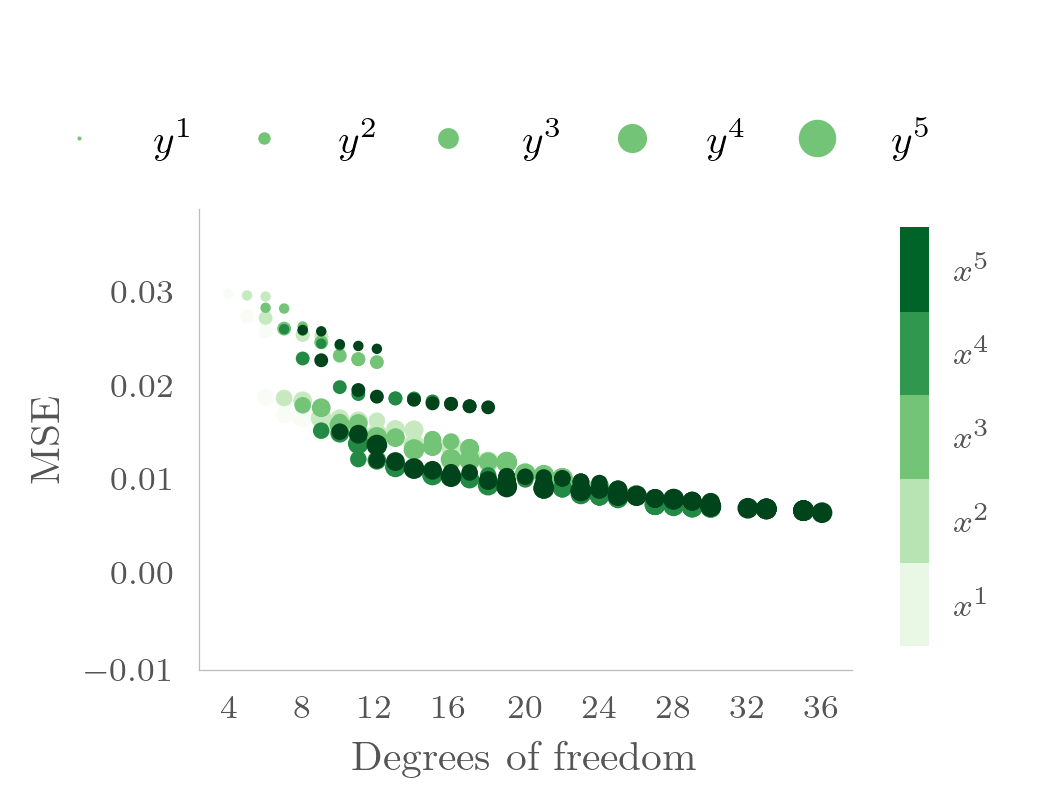
\includegraphics[]{figures/ols_group.png}
  \caption{\label{fig:olscgrouped} MSE of all models with orders up to \(x^{5}\)
  and \(y^{5}\) with all interactions. The highest order of \(x\) is visualized
  by color and highest order of \(y\) is visualized by the circle size. Since many
  models have the same degree of freedom, points overlap. The clear trend is
  that more complex models give lower MSE.\@ The test MSE is not shown.}
\end{figure}

The training MSE of running OLS on the Franke function is shown
in~\cref{fig:olscgrouped}. Polynomials up to \(5^{\text{th}}\) order was used including all possible
interactions, leading to the ``pile-up'' at a given degree of freedom. To show
the effect of increasing \(x\) and \(y\) independently, their degrees have been
visualized using color and circle radius, respectively.

As expected the training MSE is monotonically decreasing as the degrees of
freedom is increasing. This decrease is independent of whether the increase
happens in \(x\) or \(y\).

However, training error is not useful as we are unable to judge whether the
model is overfitting. To remedy this, a five fold CV is performed with the
resulting mean test MSE shown in~\cref{fig:olsmse}. In addition,  a large independent sample of
\(1000\) observations was used to test the trained models. This would not be
possible in a more realistic scenario, but here it gives an opportunity to check
how k-fold CV performs.

The training MSE behaves exactly as expected. The more the degrees of freedom,
the better the data is fitted, and the smaller the error becomes. The CV has low
variance, as can be seen from the error bars, and it too decreases as the
degrees of freedom increases.

The test error is far less optimistic, reaching a minimum at \(\approx 15\) df.
Even at lower df the error varies drastically from model to model. Once the
overfitting becomes too severe at about \(27\) df, the test MSE skyrockets off
the plot. Using the ``one standard error rule'', the optimal model uses a total
of only \(6\) degrees of freedom.

The out of sample error behaves similarly to the test error. At low df the
test error is too pessimistic, but they come to agree at around \(10\) df.
It is assuring to see that the best model chosen by the out of sample error is
the same as the test error's. 

The variance in test error and out of sample error was too large to be plotted
without creating visual clutter.

\begin{figure}
  \centering
  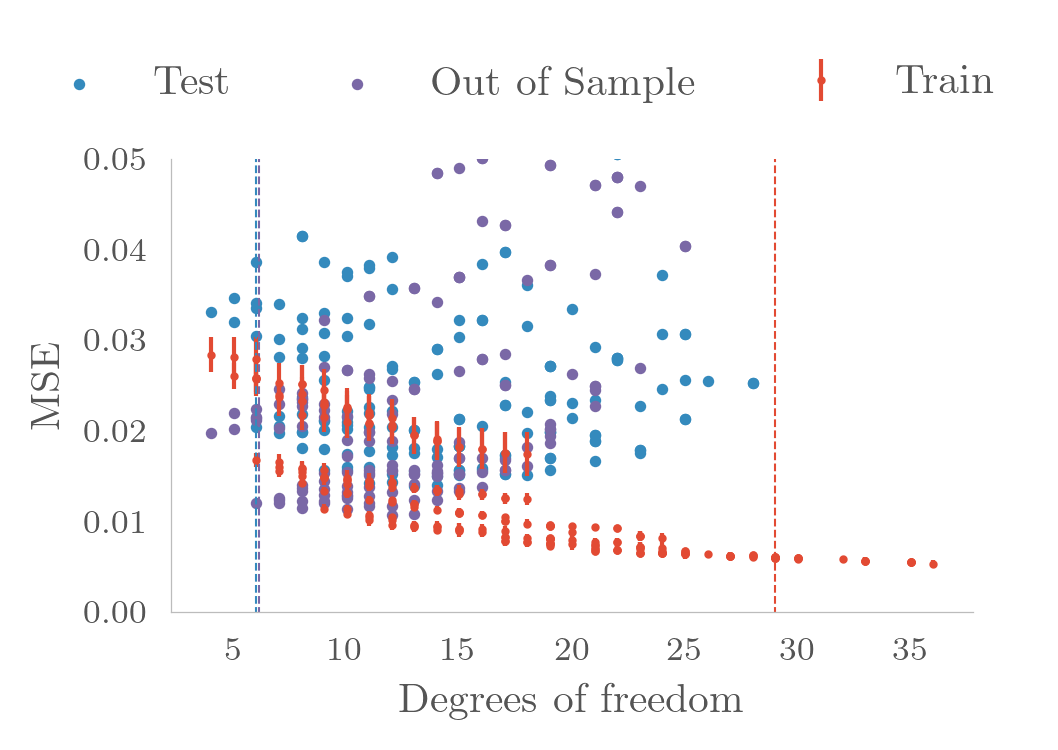
\includegraphics[]{figures/olsmse.png}
  \caption{\label{fig:olsmse} The mean square error for training, testing and
    out of sample testing using 5 fold cross validation on a sample of 100
    observations. The training error has error bars showing the CV
    distribution, while for the others the mean of the cross
    validations are shown as their variance is massive. All models of degree up to \(5\) including interactions
    are included. The outsample testing MSE is done on an independent sample of
    1000 observations. The training error is always decreasing and
    underestimating the test error. At around \(df = 20\) the models begin to
    overfit and both the test and outsample test error increases. The y-axis has
  been cut as the last points have errors two magnitudes greater. The lines mark
the best model for each error set using the ``one standard error rule''. }
\end{figure}

The \(R^{2}\) coefficient could be used to estimate the error in
our models. However, it is equivalent to a normalized version of MSE. As we are
always comparing the same data and same response, nothing is gained from using it.
For completeness, a simplified version of~\cref{fig:olsmse} using \(R^{2}\) is
shown in figure~\cref{fig:olsr2}. It tells us qualitatively the same in an
quantitative different manner, and will not be repeated in further analysis.

\begin{figure}[]
  \centering
  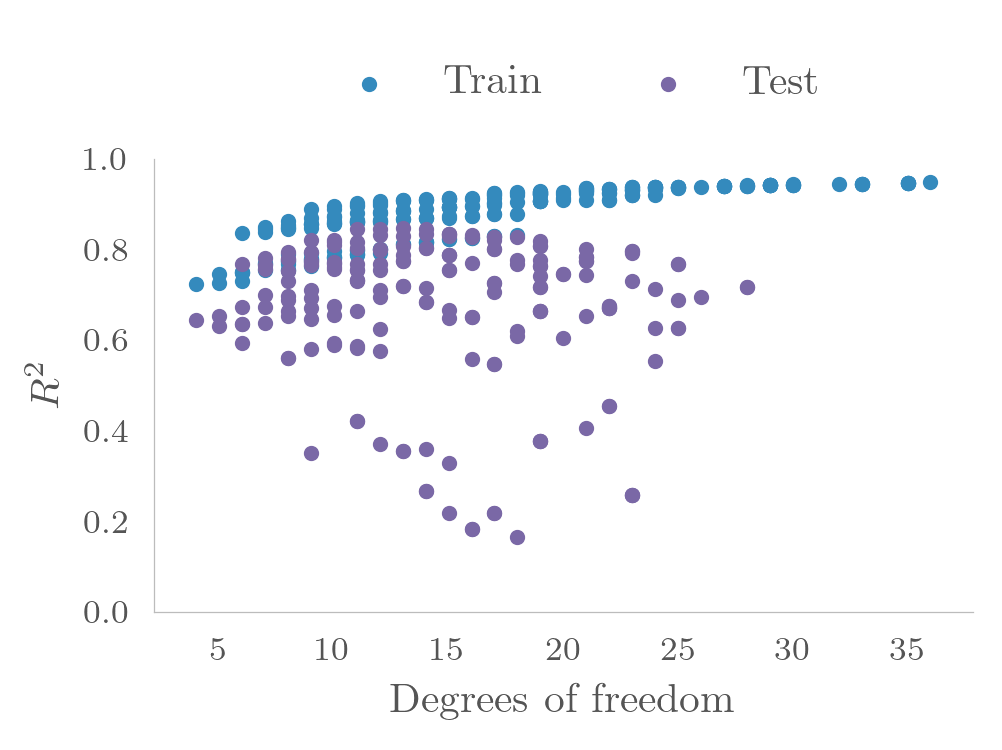
\includegraphics[ ]{figures/olsr2.png}
  \caption{\label{fig:olsr2} \(R^{2}\) coefficient plotted against degree of
    freedom of OLS for both test and training sets. It is the inverted version
    of~\cref{fig:olsmse}}
\end{figure}

In~\cref{fig:olsci} the \(95\%\) confidence intervals of the coefficients of the
best model are plotted. The constant coefficient is highly significant, and so
are the terms \(x\) and \(xy\). The remaining coefficients for \(y, y^{2}\) and
\(y^{3}\) are not as significant. This is due to the fact that they are all
correlated with each other; and increase in \(y\) is invariably followed by an
increase in \(y^{2}\) and \(y^{3}\).
\begin{figure}[]
  \centering
  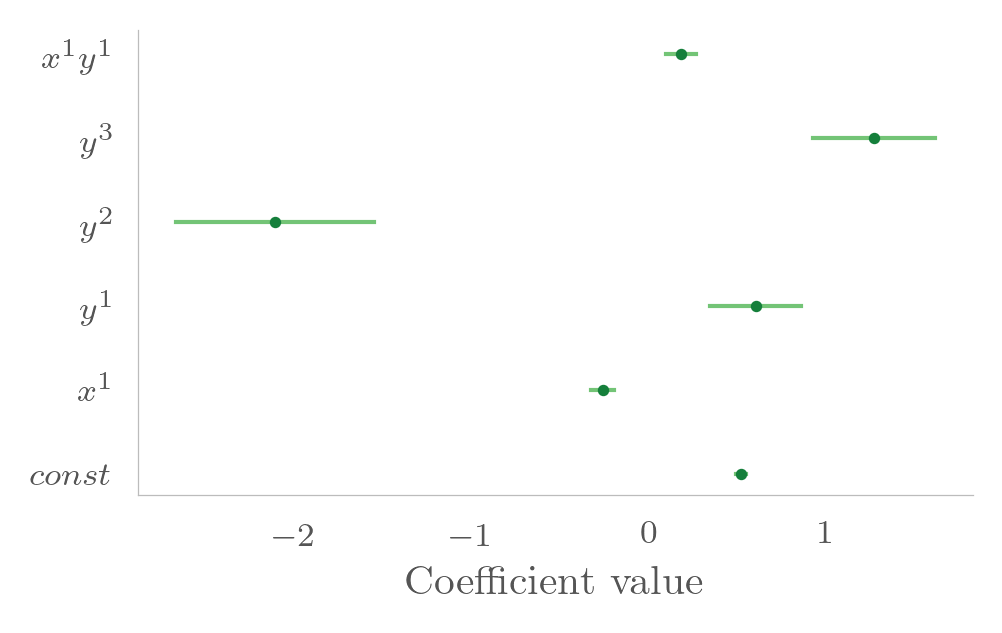
\includegraphics[]{figures/ols_ci.png}
  \caption{\label{fig:olsci} 95\% confidence interval for the best model as
    estimated by the ``one standard error'' rule for test MSE.\@ The constant and
    \(x\) term are very significant, and so is the interaction term \(xy\). all
    of the \(y\)-terms have larger CI.}
\end{figure}

A more dire picture emerges when we look at the coefficients of all models.
\cref{fig:olscoeff} shows how the coefficients diverge from zero as both the
degree of each term increases, and as the degrees of freedom increases. The most
complex terms have massive coefficients, with \(\hat\beta_{x^{5}y^{5}} \propto
-10^{5}\) and \(\hat\beta_{x^{5}y^{4}}\propto 10^{5}\).

\begin{figure}[]
  \centering
  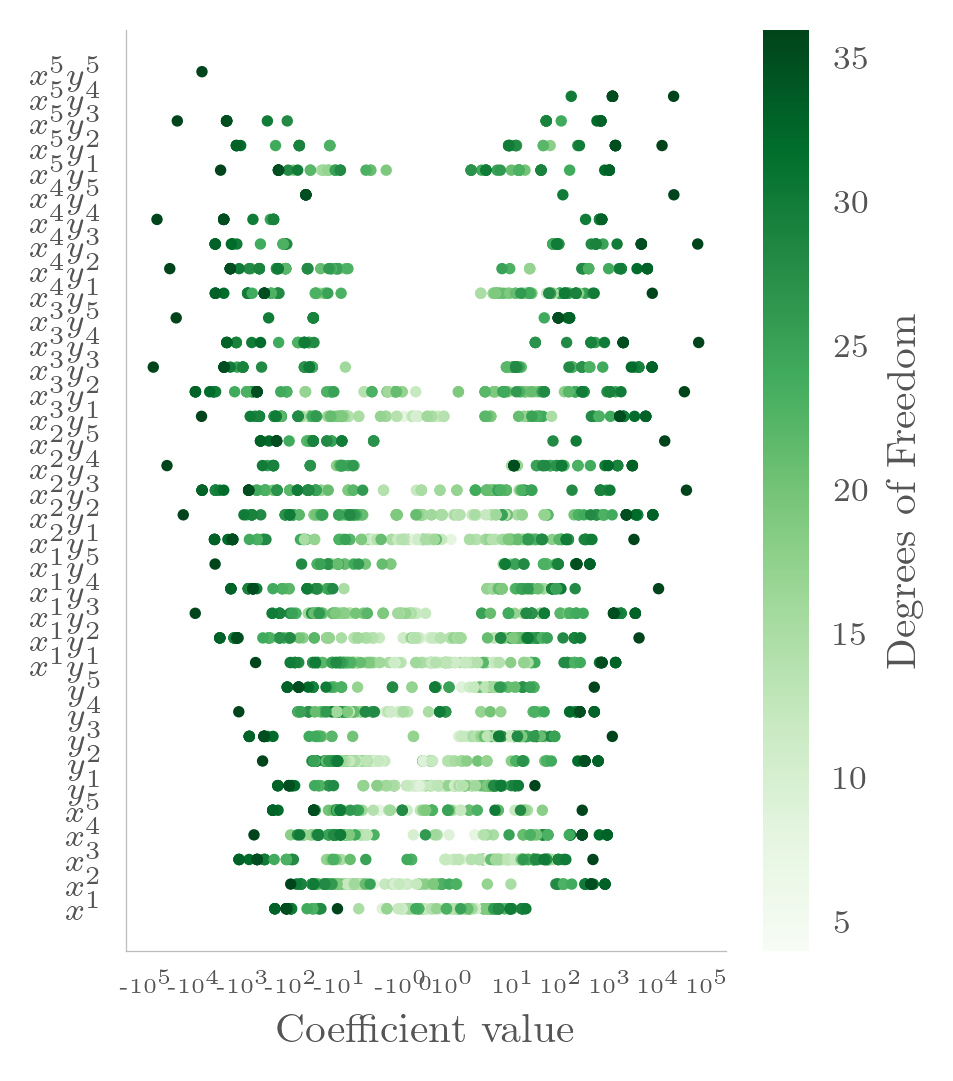
\includegraphics[]{figures/olscoeff.png}
  \caption{\label{fig:olscoeff} The coefficients for each term of each model for
  OLS.\@ As the model becomes more and more complex with larger degrees of
  freedom, the coefficients fan out, becoming highly negative or highly positive,
even switching sign from one model to the next. }
\end{figure}

Why does this happen? More insight is gained when plotting the naive, or expected
degrees of freedom \(p\) against the effective degrees of freedom
\(\text{tr}\left(\vb{H}\right)\) computed numerically. This is done 
in~\cref{fig:effectivedf}. As shown in~\cref{eq:1} the expected degrees of
freedom is \(p\), but the plot shows that this is only true for small values of
\(p\). At around \(p=15\) the computed trace begins to deviate, and it
doesn't take long before they deviate wildly. Almost unequivocally, the
effective degrees of freedom is lower than the expected values. This can be
interpreted as the design matrix containing less information than what is
expected.

\begin{figure}[]
  \centering
  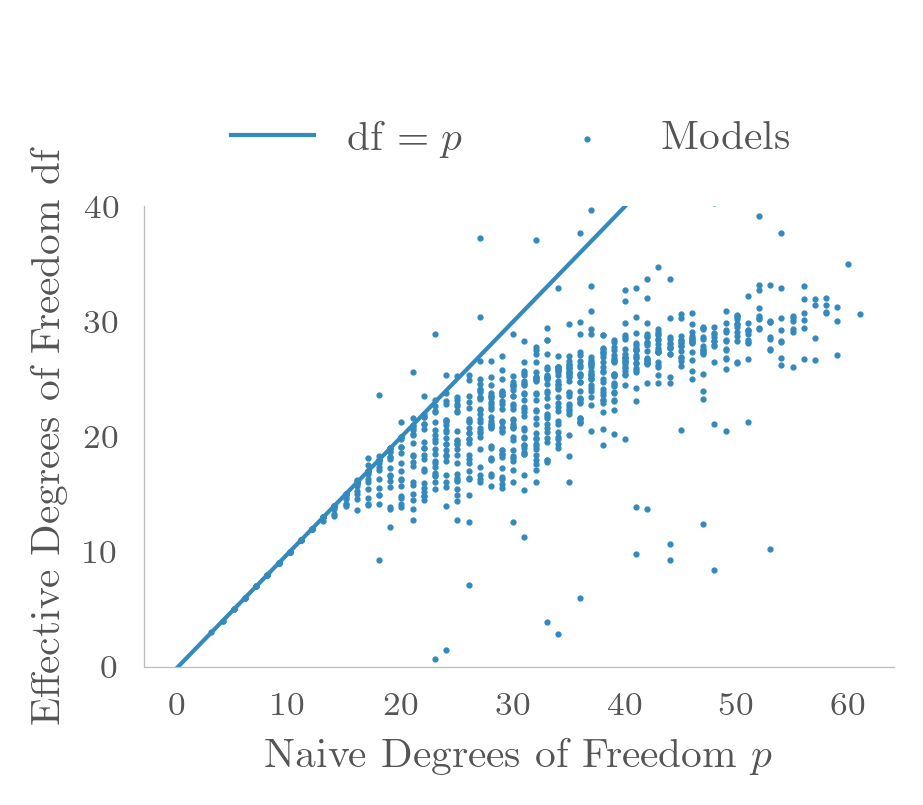
\includegraphics[]{figures/effectivedf.png}
  \caption{\label{fig:effectivedf} Effective degrees of freedom computed
    numerically as the trace of \(\vb{H}\) versus the expected degrees
    of freedom \(p\). For high \(p\) the effective degrees of freedom deviate,
    becoming progressively lower.}
\end{figure}

Taking another look at~\cref{eq:1}, the culprit seems to be matrix inversion of
\(\vb{X}^{T}\vb{X}\). If this matrix is ill conditioned, the inversion will
be ill conditioned, and the computed trace of \(\vb{H}\) can not be taken
seriously. Indeed, when the condition number of \(\vb{X}^{T}\vb{X}\) is plotted
for increasing \(p\), it is clear that the matrix is ill conditioned.
See~\cref{fig:condition}.  

\begin{figure}[]
  \centering
  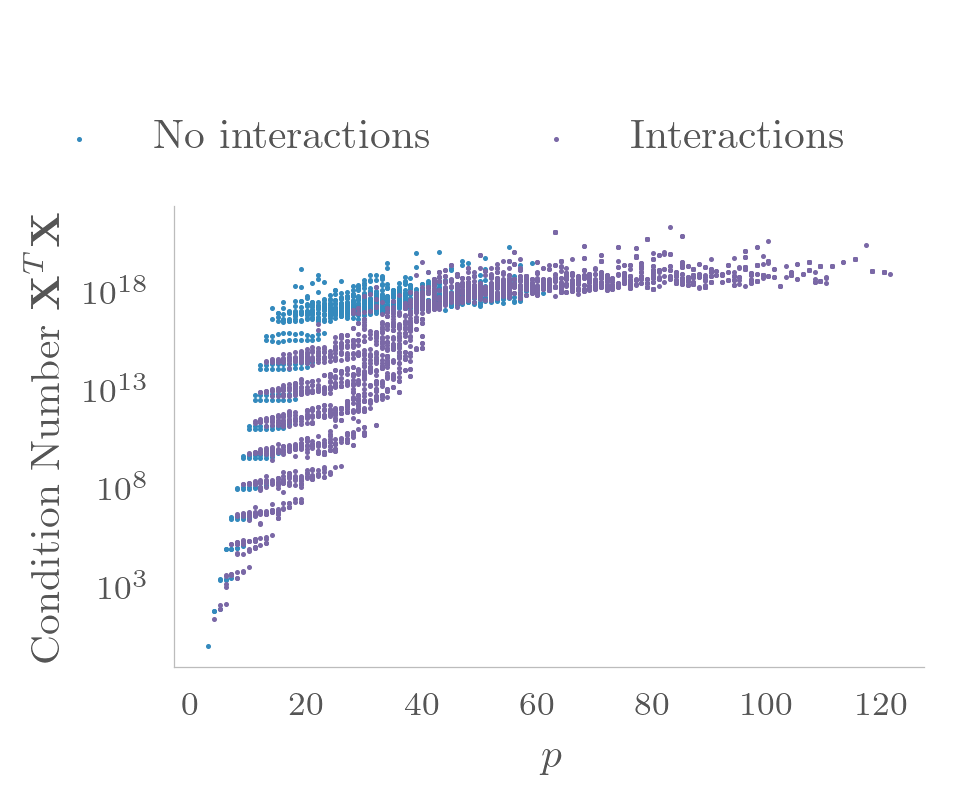
\includegraphics[ ]{figures/condition.png}
  \caption{\label{fig:condition} Condition number of the matrix
    \(\vb{X}^{T}\vb{X}\) for larger \(p\), i.e. more columns. A matrix with
    interactions follows the same pattern as one without, constantly increasing
    for larger \(p\). The apparent plateau at \(10^{18}\) is due to the y-axis
    being restricted as terms blow up to \(10^{50}\)}
\end{figure}

Now the question becomes: \textit{why} is the matrix \(\vb{X}^{T}\vb{X}\)
ill-conditioned? We have already seen that correlation between coefficients
increases their confidence interval, so correlation between the columns in
\(\vb{X}\) is suspect.

Plotting Pearson correlation coefficient between each
term in~\cref{fig:correlation}, the suspicion is confirmed. As the highest
degree of \(x\) and \(y\) increases, and as the number of interactions
increases, the greater the correlation. The greater the correlation, the more
similar are the columns of \(\vb{X}\), and the smaller its column space becomes.
This makes inversion of \(\vb{X}^{T}\vb{X}\) more and more ill-conditioned, and
the effective degrees of freedom becomes smaller and less reliable. In practice,
this means that terms that are highly correlated will have coefficients that are
similar but with opposing signs to cancel each other out, contributing little to
the explaining power of the model in question.

\begin{figure}[]
  \centering
  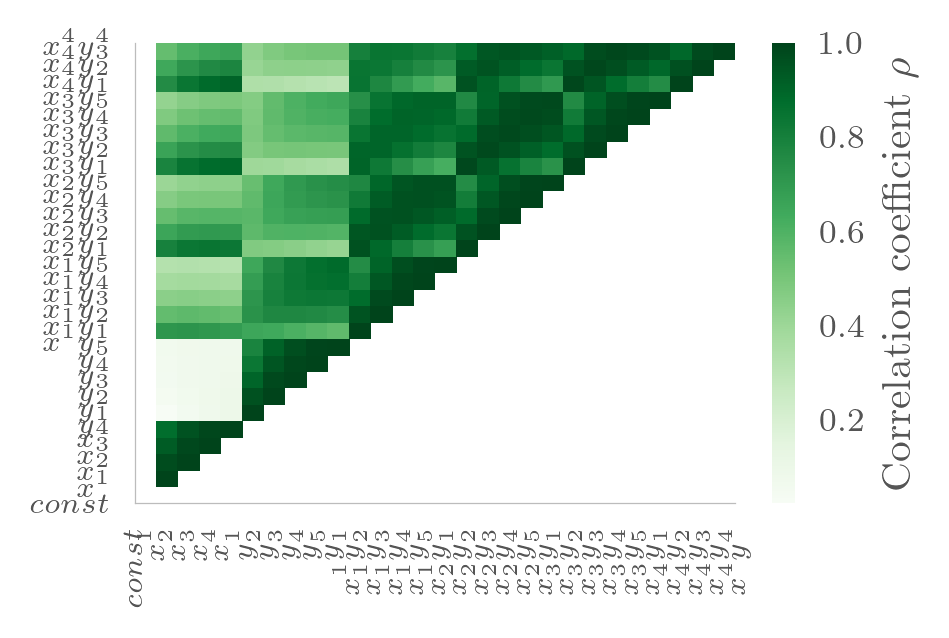
\includegraphics[ ]{figures/correlation.png}
  \caption{\label{fig:correlation} Correlation matrix for each term of the
    design matrix. The higher the degree, the higher the correlation with almost
  all other terms, especially for the interaction terms.}
\end{figure}


\subsubsection{Ridge Regularization}
\label{sec:ridge-regularization}

Ridge regularization steps in as the savior of ill-conditioned matrices. Adding
\(\lambda \vb{I}\) to \(\vb{X}^{T}\vb{X}\) greatly reduces the
condition number, as seen from~\cref{fig:condridge} with \(\lambda = 0.01\). We
can therefore be more confident in the numerical stability of the Ridge estimates.

\begin{figure}[]
  \centering
  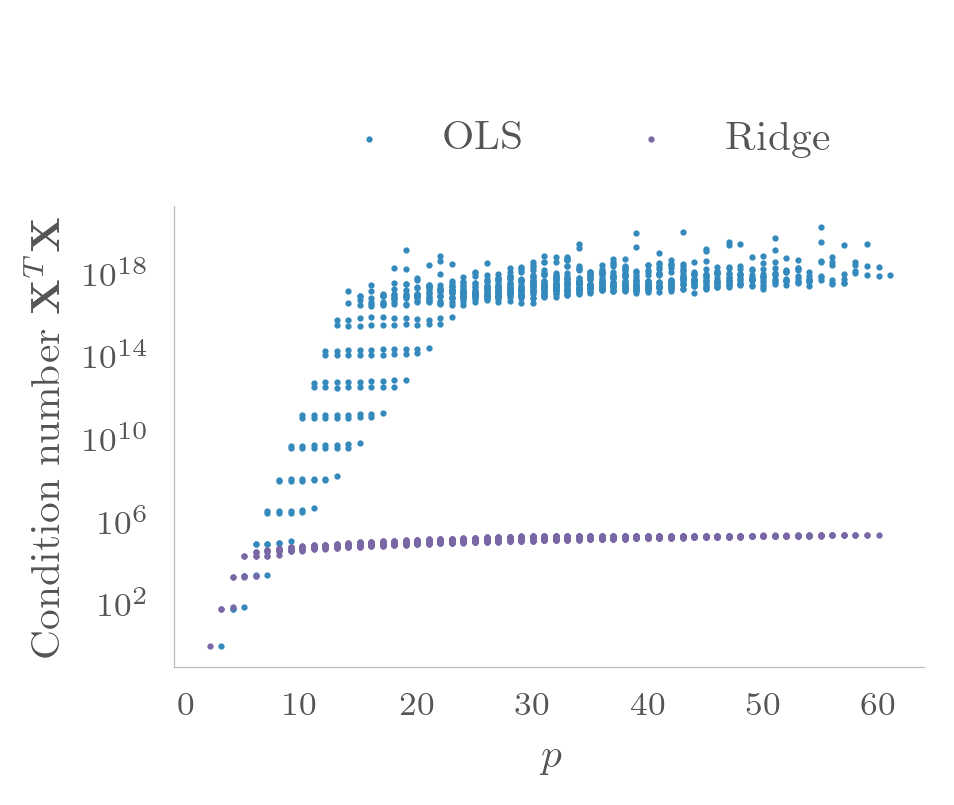
\includegraphics[ ]{figures/condition_ridge.png}
  \caption{\label{fig:condridge} Condition number of \(\vb{X}^{T}\vb{X} +
    \lambda\vb{I}\) plotted against number of
    columns \(p\) in \(\vb{X}\). The OLS has \(\lambda = 0\) and experiences
    larger condition numbers for larger \(p\). Ridge uses \(\lambda = 10^{-2}\)
    causing the matrices to be better conditioned with the condition number
    leveling off at \(p\approx 10\)}
\end{figure}

For modeling the Franke function the maximal model of degree \(5\) using all
interactions is fitted for a range of \(\lambda\)s. The same analysis performed
on OLS is repeated and shown in~\cref{fig:ridgemse}. Increasing the
\(\lambda\) from \(0\) initially causes the MSE to rise and increase variability
of the cross validation samples before falling and causing train, test and out
of sample MSE to converge. Again the test and out of sample agrees on the best
model using \(\lambda \approx 5\times 10^{-2}\).

\begin{figure}[]
  \centering
  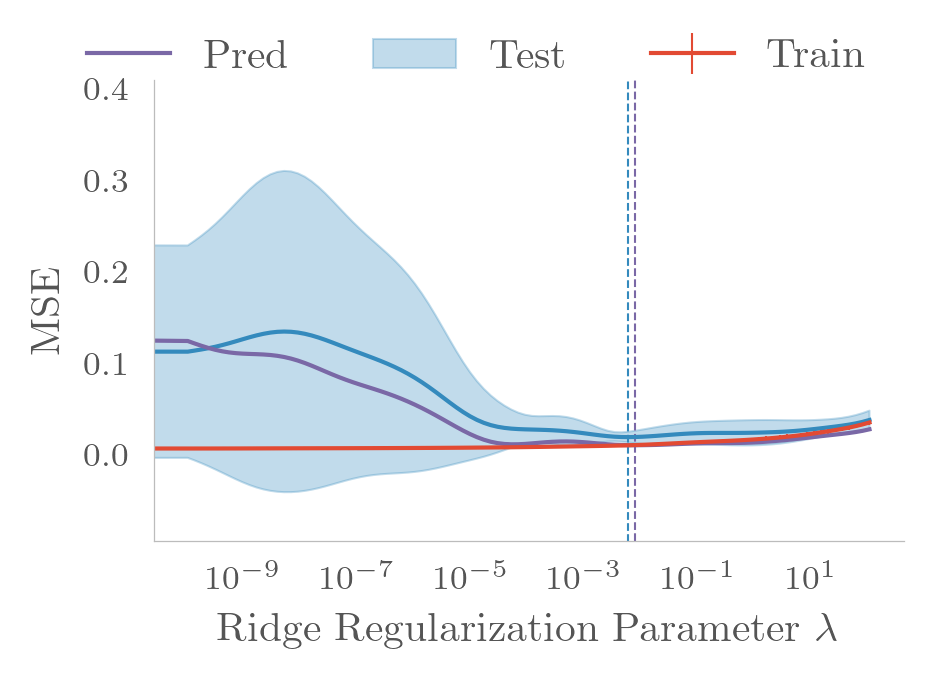
\includegraphics[]{figures/ridgemse.png}
  \caption{\label{fig:ridgemse} The MSE of Ridge regression as a function of
    hyperparameter \(\lambda\). In the beginning the variability is high, but
    decreases quickly to a significant minimum at \(\lambda\approx 5\times
    10^{-2}\)  in agreement with the out of sample error \textit{Pred})}
\end{figure}

Ridge regularization penalizes large coefficients, as can be seen
by~\cref{fig:ridgecoeff} and~\cref{fig:ridgecoeffevo}. As \(\lambda\) increases,
all of the coefficients decrease, but the large coefficients shrink the
fastest. In addition there are no longer any large-but-opposite coefficients
that the OLS was plagued by, visible from the lack of the ``fan'' pattern of coefficients
at large term degrees. 

As \(\lambda\) increases, coefficients sometimes rises after being shrunk, or
changing sign, as is seen in the lower symlog-plot
in~\cref{fig:ridgecoeffevo}. This is due to the collinearity between the terms.
As one term is decreased, the variance it explained can be given to one of its
correlated variables, causing them to increase or change sign. This dance
between the coefficients happens no matter the value of  \(\lambda\).


\begin{figure}[]
  \centering
  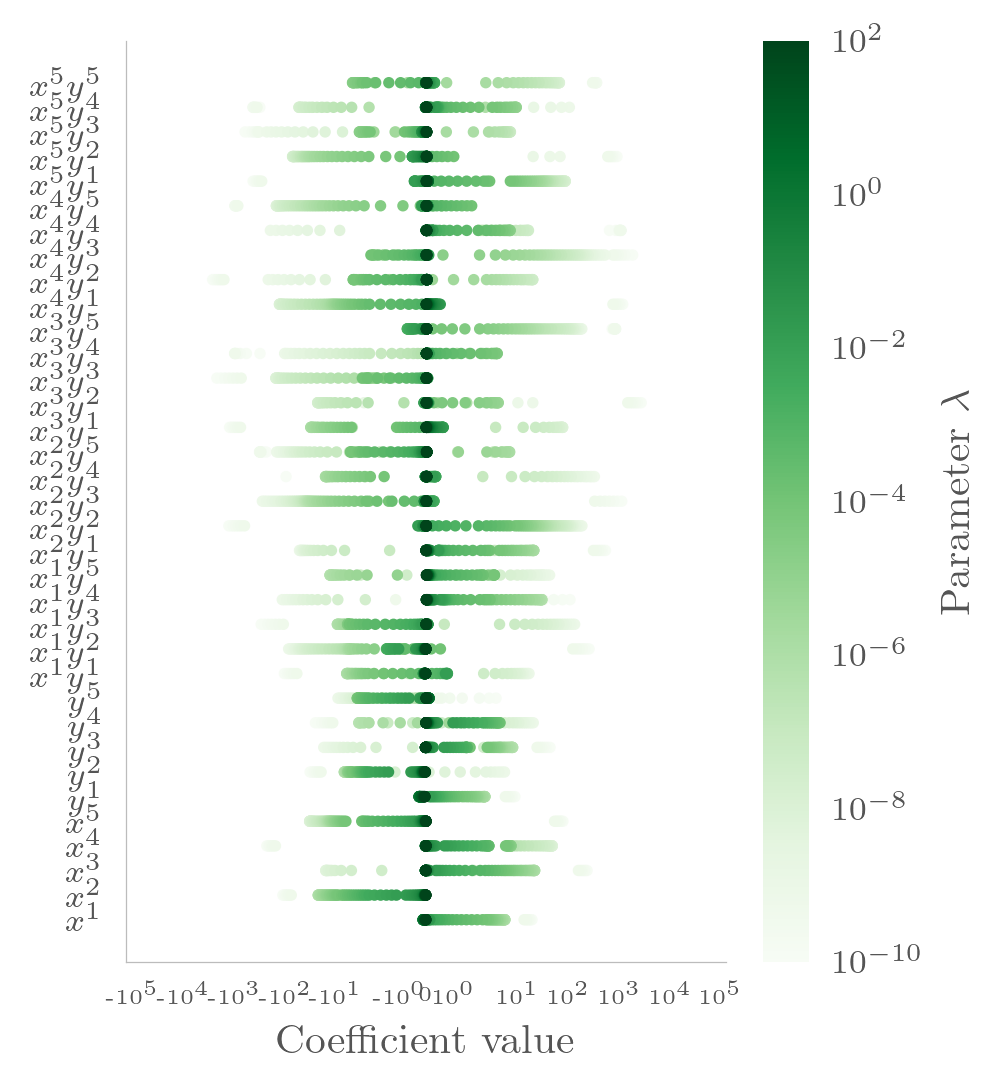
\includegraphics[ ]{figures/ridgecoeff.png}
  \caption{\label{fig:ridgecoeff}  As the Ridge regularization parameter
    \(\lambda\) increases all terms are penalized and shrunk towards zero. The
    plot is symmetric about zero, showing that the coefficients change sign from
  time to time.}
\end{figure}

\begin{figure}[]
  \centering
  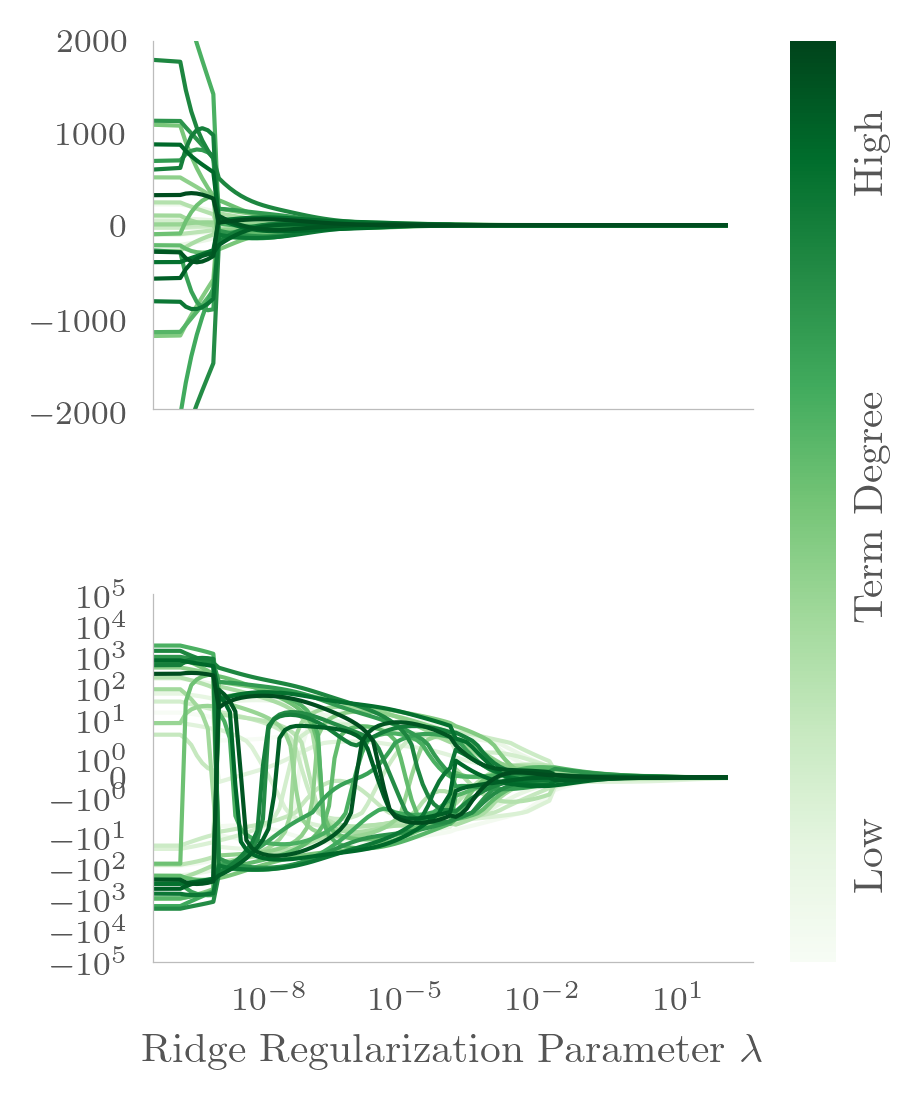
\includegraphics[ ]{figures/ridgecoeff_evo.png}
  \caption{\label{fig:ridgecoeffevo} The coefficient of each term plotted
    against the Ridge hyperparameter. The top plot uses a linear scale to show
    how fast the large coefficients are shrunk to zero even with a zoomed in
    y-axis, while the more intricate behavior is seen in the lower plot user
    symmetric logarithmic y-axis. The lower degree terms are smaller and shrunk
    slower than the higher degree terms. The higher terms also have large
    collinearity, causing them to dance around zero as their explained
    variability is explained by other correlated coefficients.}
\end{figure}

\subsubsection{Lasso Regularization}

The regularization methods of Ridge and Lasso are so very similar, yet their
effects are surprisingly different. Performing the identical analysis as done
with Ridge gives the MSE in~\cref{fig:lassomse}. Instead of decreasing the MSE
as Ridge, the MSE is continually increased for larger \(\alpha\). When
\(\alpha\) gets sufficiently large at \(\alpha>0.1\), the error plateaus. As a
result, the test MSE recommends the smallest \(\alpha\) available. In contrast, the out of sample MSE
recommends a small regularization at \(\alpha\approx 8\cross 10^{-2}\). Weirdly enough, the out of sample
MSE is consistently \textit{below} both the test and training MSE.\@ It is unknown
why this happens.

\begin{figure}[]
  \centering
  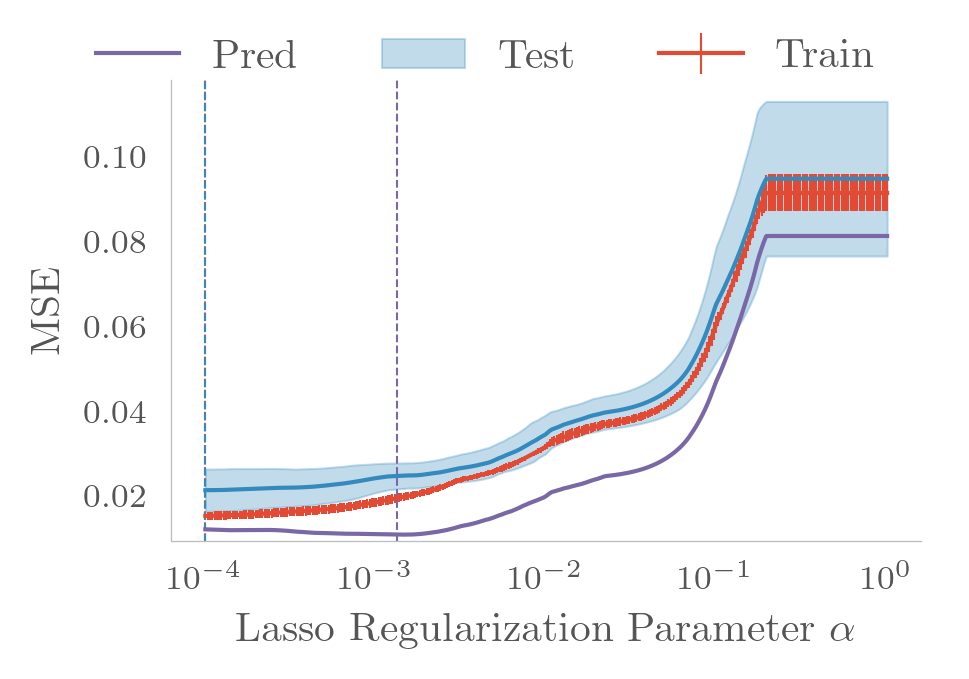
\includegraphics[ ]{figures/lassomse.png}
  \caption{\label{fig:lassomse} The MSE of Lasso regression as function of
    hyperparameter \(\alpha\). In contrast to Ridge~\cref{fig:ridgemse} neither
    the test MSE or training MSE decrease with any significance. Once the
    hyperparameter gets too large, all terms are set to zero, causing the error
    to plateau. The out of sample error \textit{Pred} is confusingly enough
    smaller than both test and training error.}
\end{figure}

Another difference from Ridge is that the large coefficients quickly gets set to
zero, as seen from~\cref{fig:lassocoeff} and~\cref{fig:lassocoeff_evo}. The
terms of smaller degree experience a smaller penality, thus staying larger over
larger ranges of \(\alpha\). The coefficient plot gains an ``inverted V'' shape
in contrast to OLS' fan shape and Ridge's uniform shape.

As \(\alpha\) is increased, the number of coefficients set to exactly zero increases rapidly.
\cref{fig:zeros} shows the total number of zeros. At \(\alpha=10^{-4}\), six
coefficients are already zero, while at \(\alpha\gtrsim 0.1\) \textit{all}
coefficients are set to zero, explaining the MSE plateau.

\begin{figure}[]
  \centering
  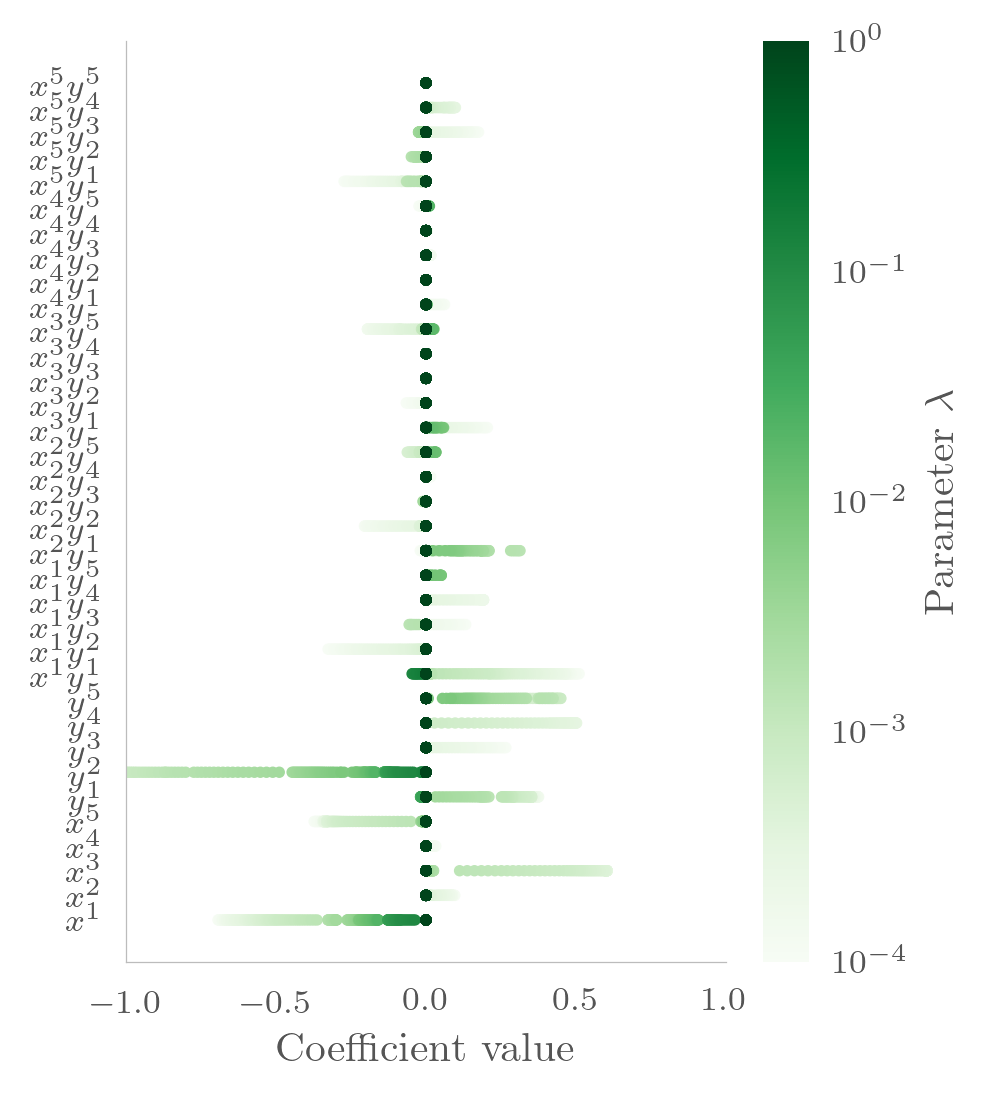
\includegraphics[ ]{figures/lassocoeff.png}
  \caption{\label{fig:lassocoeff} The coefficient of each term as the Lasso
    regularization parameter increases. The highest terms are penalized more
    heavily than the low, causing them to quickly go to zero. Note also the
    jumps that happen when a term is temporarily set to zero before being turned
  on again later. Note the scale different of the x-axis compared to~\cref{fig:ridgecoeff}}
\end{figure}

\begin{figure}[]
  \centering
  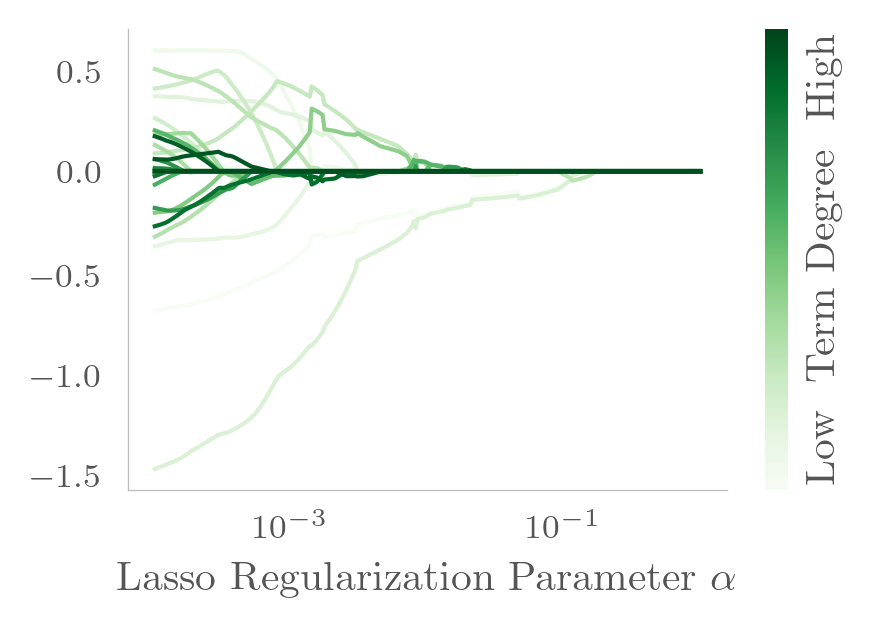
\includegraphics[ ]{figures/lassocoeff_evo.png}
  \caption{\label{fig:lassocoeff_evo} The evolution of the coefficients as
    function of increasing Lasso hyperparameter \(\alpha\). In the beginning all
    many high terms have been heavily penalized or set to zero, giving the
    apparent ``inversion'' of colors when compared to~\cref{fig:ridgecoeffevo}.
    The coefficients also do not cross the zero line in contrast to Ridge.}
\end{figure}

\begin{figure}[]
  \centering
  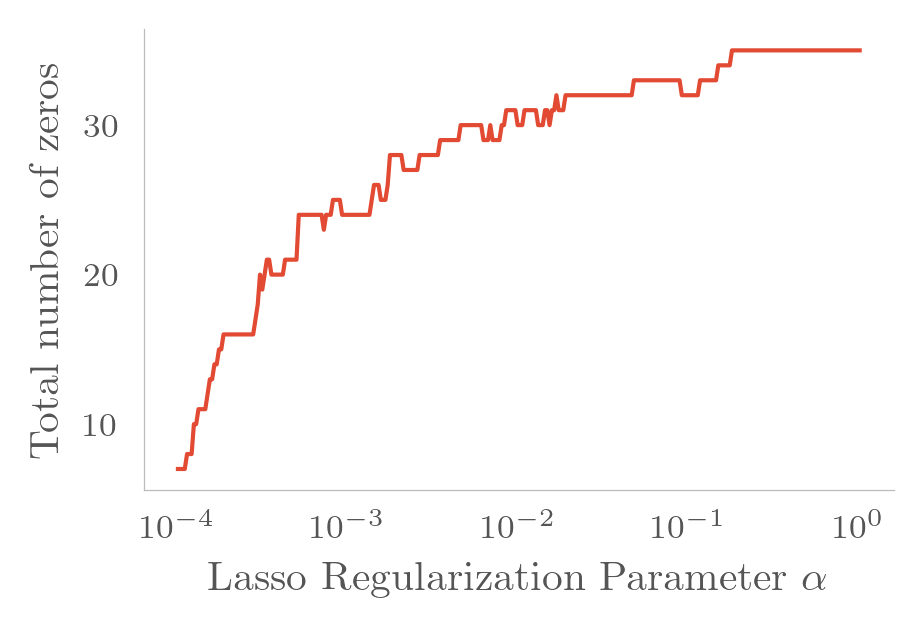
\includegraphics[ ]{figures/zeros.png}
  \caption{\label{fig:zeros} The relationship between the total number of terms
    set to zero to the increasing regularization parameter. Even at very low
    \(\alpha\) some terms are set to zero. For high \(\alpha\) all terms are set
    to zero.}
\end{figure}


\subsection{Comparison}

Predictions based on OLS, Ridge and Lasso for the Franke function are shown in
\cref{fig:compare}. For the sample size we have used, \(100\) observations, the
amount of features found in the Franke function that can be captured by the
models is not impressive.

The OLS training manages to capture the two hills and one valley, but at the
cost of huge boundary effects. The OLS test model fails at capturing any single
feature, instead opting to smudging the two hills into one slope and the one
valley into a long shallow one.

Ridge and Lasso gives higher order terms ability to express themselves, which is visible
in the clearer outlines of the features. Lasso has the added benefit of setting
some coefficients to exactly zero, and from the plots it has better behaved
boundaries.
\begin{figure}[]
  \centering
  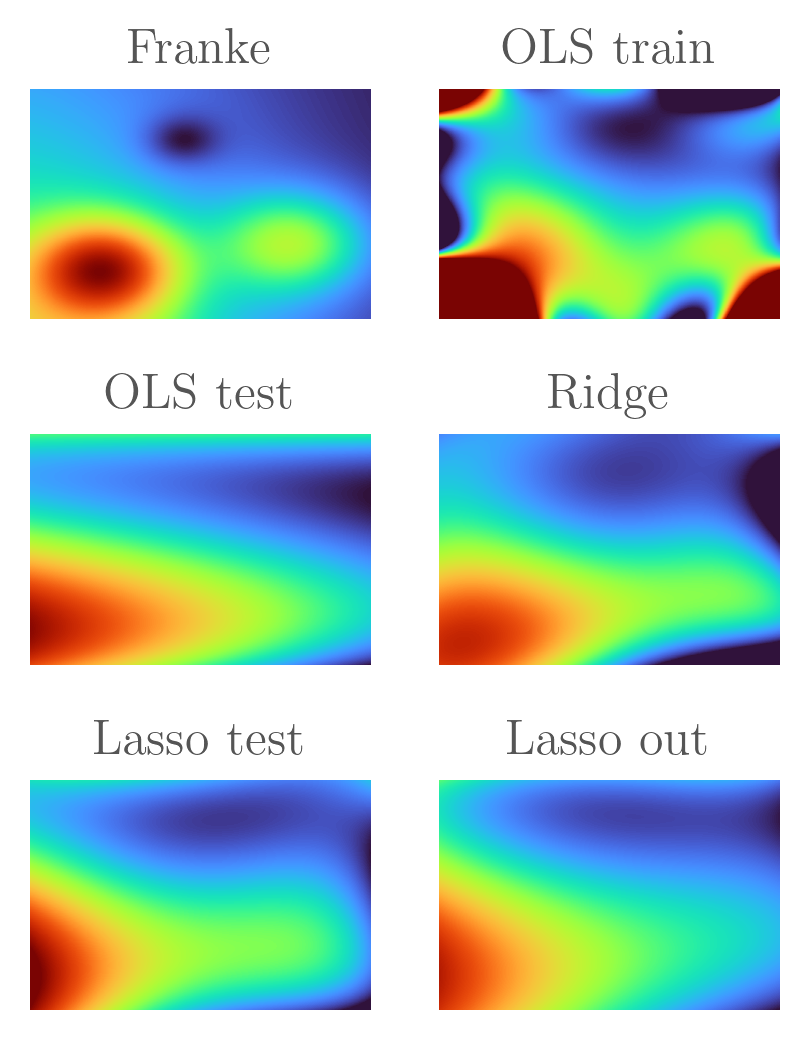
\includegraphics[ ]{figures/comparisons.png}
  \caption{\label{fig:compare} Comparisons of the different regression methods
    applied to the Franke function. The Franke function is shown in the top
    left. The OLS training has overfitted, giving good fit for a few regions
    while others are utterly wrong and the boundaries goes to infinity. The OLS
    test is much more conservative, using a low degree polynomial. Ridge
    penalizes the higher coefficients while still retaining their explaining
    power, hence better at recreating the features of the Franke function. Some
    boundary issues are seen on the right edge. The Lasso test MSE recommends
    the smallest possible \(\alpha\) while the out of sample MSE prefers a
    higher \(\alpha\), their results shown at the bottom. The  higher \(\alpha\)
    causes features of the plot to be more washed out.}
\end{figure}

\subsection{Terrain Data}

The real world terrain data has much, much more features than the Franke
function, so to make the problem somewhat solvable, the terrain is downsampled
and \(300\) observations are drawn. OLS, Ridge and Lasso are run, and their MSE
plots shown in figures~\ref{fig:geo_reg_mse}, \ref{fig:geo_ridge_mse},
and~\ref{fig:geo_lasso_mse}. Behavior similar to the Franke function is seen. For
OLS, the training MSE falls just as before and test MSE has a small dip before
it increases. For Ridge the behavior is similar, but with a huge error and
variance at very low parameter values. This is probably due to the fact that the
Ridge and Lasso start out with 15 degree polynomials, and are prone to
overfitting at low parameter values. The error quickly drops, however, and the
test error reaches a minimum at a \(\lambda \approx 0.9\). The Lasso error again
prefers a low value of \(\alpha\), rising to a plateau for large
\(\alpha\) and being unchanged over the intermediate range.


\begin{figure}[]
  \centering
  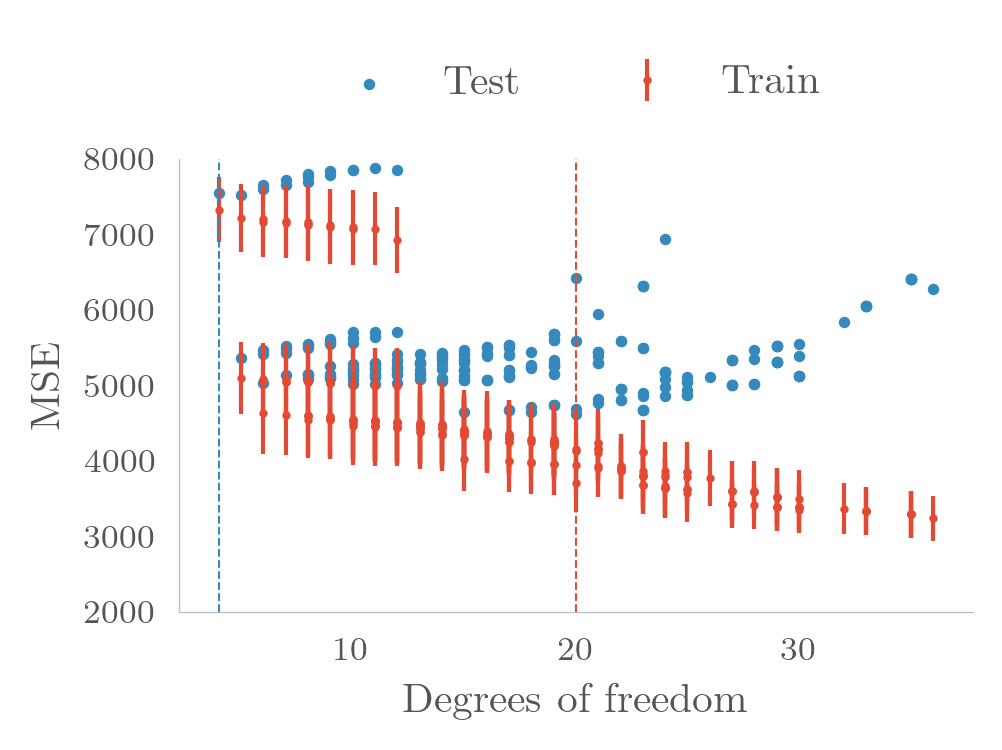
\includegraphics[ ]{figures/geo_reg_mse.png}
  \caption{\label{fig:geo_reg_mse} Training and test MSE of ordinary least
    squares regression using \(100\) observations of the downsampled terrain.
    Note the contrast error bars of the training data to the error bars
    in~\cref{fig:olsmse} indicating data with higher variance. This causes the
    best training model to be more conservative, not choosing the one with most
    terms. The variance of the test data is very large, so the significantly
    best model is the simplest possible}
\end{figure}

\begin{figure}[]
  \centering
  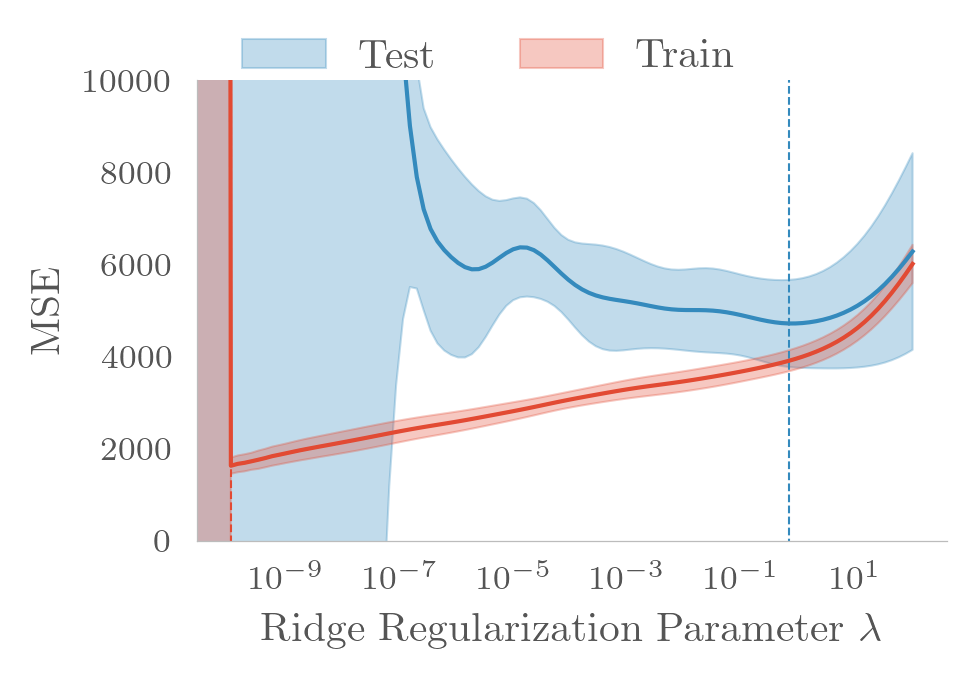
\includegraphics[ ]{figures/geo_ridge_mse.png}
  \caption{\label{fig:geo_ridge_mse} The MSE of Ridge as a function of
    regularization parameter for the downsampled terrain using \(15\) degree
    polynomials with all interactions. For low values the model overfits, giving
    an enormous spike with high variability. The situation improves for
    \(\lambda > 10^{-5}\) with the test MSE giving the optimal model at
    \(\lambda\approx 0.9\) before increasing once the penalty decreases the
    coefficients too much.}
\end{figure}
\begin{figure}[]
  \centering
  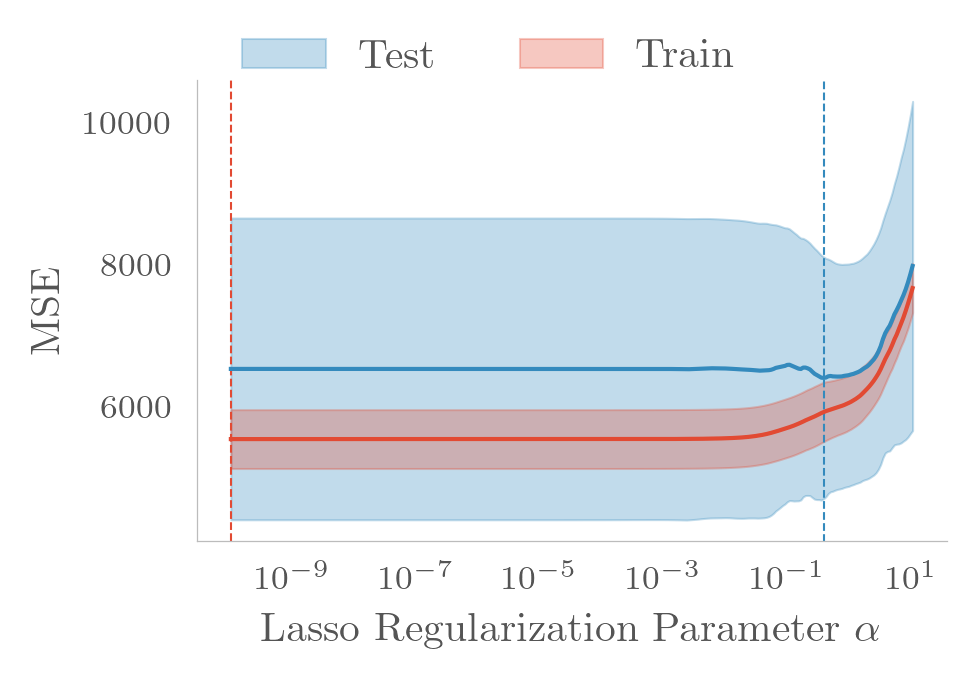
\includegraphics[ ]{figures/geo_lasso_mse_2.png}
  \caption{\label{fig:geo_lasso_mse} The MSE of Lasso as a function of
    regularization parameter for the downsampled terrain using \(15\) degree
    polynomials with all interactions. Even at very small parameter values the
    largest coefficients are set to zero. Afterwards increasing the parameter
    has very little effect before too many coefficients get set to zero and the
   MSE rises. As a result, the optimal model uses the smallest possible value of
 \(\alpha\). The plateau coming up on the right is left out of the plot}
\end{figure}

The best model of each is shown in~\ref{fig:geocomp}, and again we see
similar behavior to the Franke modeling. The best OLS training is more
conservative than before due to the higher model variance, and does not have as severe boundary issues, while the OLS test
model is much more conservative and barely gives a recognizable outline. 

Both Ridge and Lasso fares better, both managing to capture the mountains in the
north-west and outline of the coast while having no boundary issues. Yet the
result is disappointing. To snuff out any hope that a higher order OLS could
perform better, a \(20\) degree fit with all interactions and \(1000\)
observations are shown in the final facet. While it manages to capture some
features, there are many phantom features that do not exist in the data, and the
boundaries are utterly wild.

\begin{figure*}[b]
  %\centering
  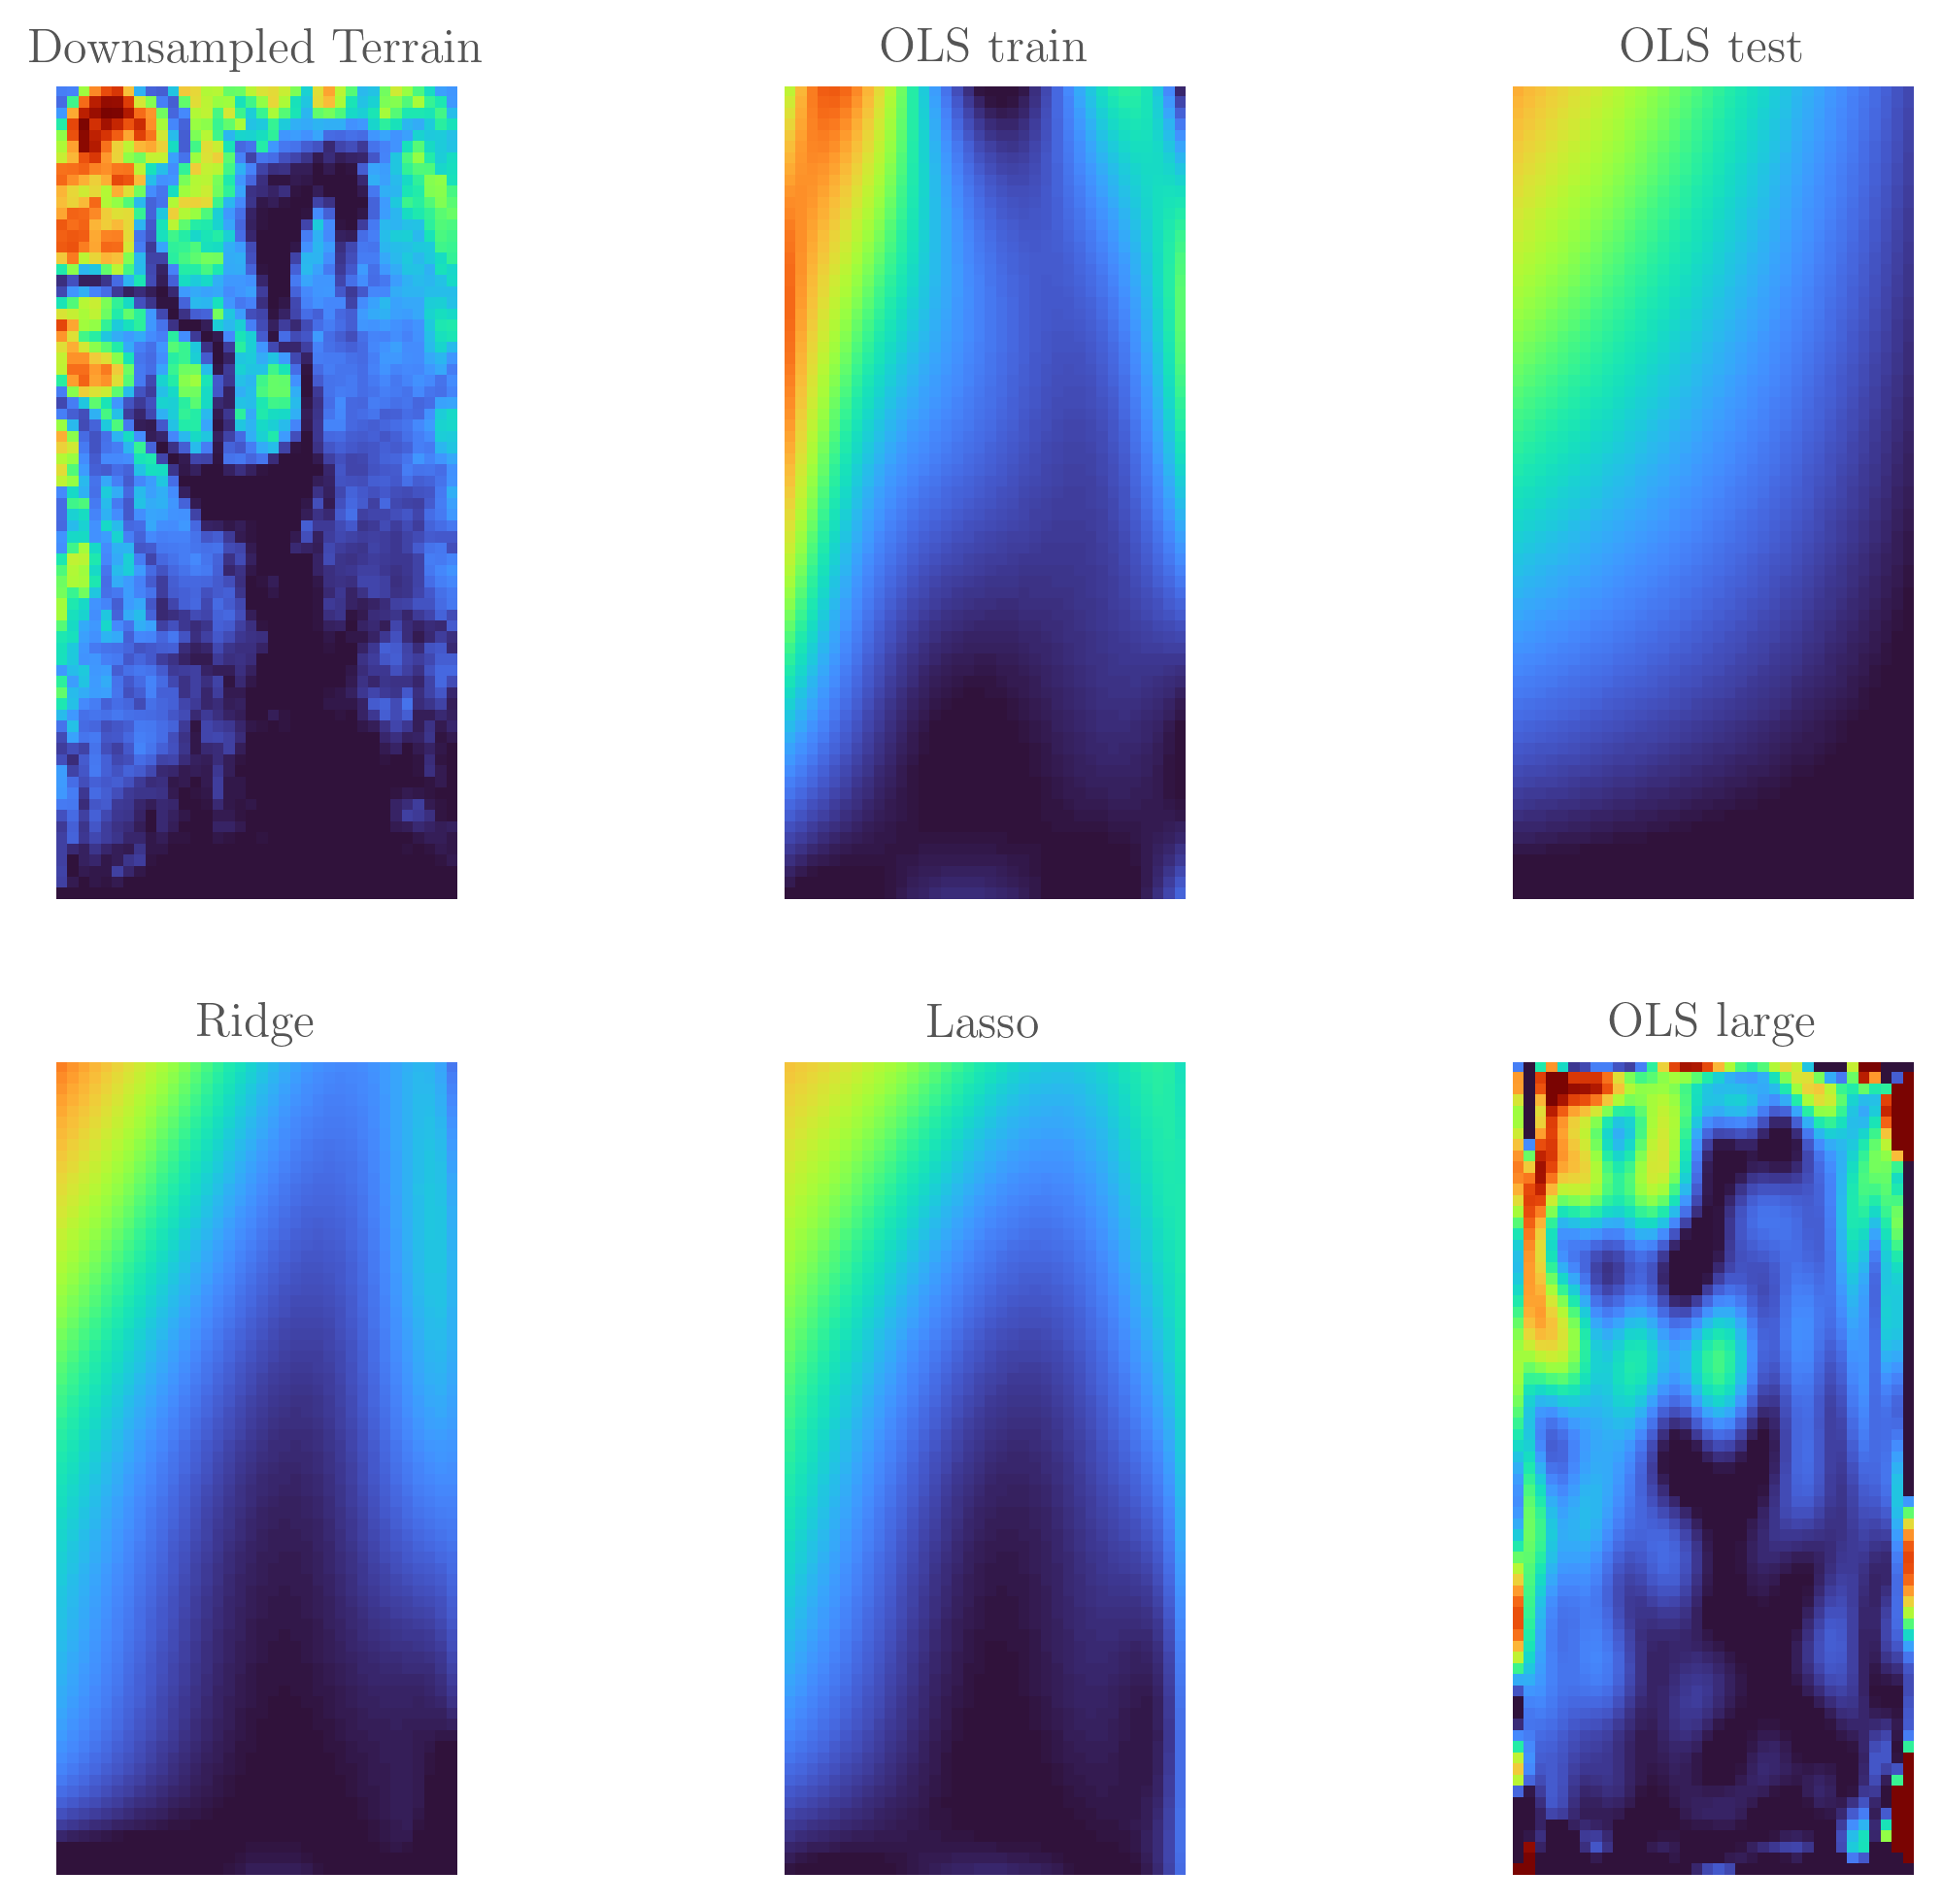
\includegraphics[]{figures/geo_comp.png}
  \caption{\label{fig:geocomp} Comparison of the best models according
    to the ``one standard error'' rule. The models were trained on the
    downsampled terrain shown in the first panel to the top left. The first two
    OLS panels were selected from polynomials up to degree \(5\), while Ridge
    and Lasso used only degree 15 while selecting from different values of their
    hyperparameters. The last panel to the lower right used polynomials of
    degree 20 with all interactions and \(1000\) observations in contrast to the
  others' \(100\). Even in its downsampled incarnation, the terrain has many
  features that the model are unable to capture. Only the mountains to the north
west and the coast lines are captured.}
\end{figure*}

There is a tradeoff between a model's ability to fit the terrain and
overfitting, in this case more severe that one would naively expect. To fit the
terrain features to any satisfying degree, a very high polynomial degree is
needed. This in turns gives a ill-conditioned design matrix, giving high
numerical instability in the predictions of the model, and boundary problems. To
remedy this regularization is introduced, but this very process shrinks the
high degree terms as these are the ones which are the most correlated. This
reduces the model's ability to describe finer details, and the explaining power
of the model decreases. If we try to increase the number of observations to
better fit the model, then we have to increase the resolution, and more
minute terrain features appear which the model already have difficulty fitting. A proper catch-22.

What, then, is the optimal solution? If the problem is to describe a terrain, then the
approaches described here are ill-suited. No choice of polynomial degree and
regularization parameter will be sufficient while still having enough data to fit the
model.

If we instead would want to compress the image data by using polynomials
reminiscent of JPEG's Fourier decomposition, these approaches are also
ill-suited. To get enough terms to catch features to a satisfying degree will
increase the number of coefficients, and storage of these coefficients will
quickly demand more space than simply storing the raw image data themselves. A
downsampled image would be much better suited. However, if one would insist to
use polynomial regression to compress the image, then using Lasso would be the
best solution as this will set many coefficients to exactly zero, meaning less
data to store. 

A possible application of polynomial regression to terrain data is to
quantitatively describe the ``roughness'' of the terrain. By using a
standardized polynomial, fitting a terrain and computing the \(R^{2}\), we
obtain a standardized measure for how rough the terrain is. A flat terrain will
be easier to fit using a low degree polynonimal than a rough terrain, and
therefore have a higher \(R^{2}\).

For these problems the only interest is in the models' ability to explain the data, not their
predictive power nor their ease of interpretability. Increasing the model
complexity would therefore be desired, if it had not been for the greater
numerical instability.

As one of the main problems with this method is the high collinearity between
the columns of the design matrix, a venue of future exploration is to either
orthogonolize the matrix or construct it using orthonormal polynomials, such as
Chebyshev polynomials. 